\documentclass{article}
\usepackage{amsmath}
\usepackage{amssymb}
\usepackage{tabularx}
\usepackage{amsmath}
\usepackage{graphicx}
\usepackage{systeme}
\graphicspath{ {./diagrams/} }

\begin{document}
\setlength{\parindent}{0in}

\begin {center}
\large Thesis
\end{center}

\section{State of the art}
\subsection{Similar Games}
\subsubsection{Keep Talking and Nobody Explodes}
The game consists in defusing a ticking bomb by solving puzzles attatched to it. It's a two player game, one player is the defuser and the other has a bomb-defusal manual. The players have to exchange the puzzle descriptions and solutions. 
\subsubsection{Unrailed}
The game consists in constructing a railway in front of a moving train. If the trains runs out of track, the game is over. In order to construct rails, the players have to chop trees, mine stone and combine materials in a specialized train cart. It's a 2 to 4 player game. The players  usually talk to split tasks among themselves and get time-sensitive tasks done quickly.
\subsubsection{Among Us}
The game is a mafia game between two teams, impostors and crewmates. A team wins if the other team is dead, crewmates also win when they complete all tasks. Impostors may kill crewmates. If a crewmate finds a corpse, he may call a vote. The player who has to most votes is killed. The players have to discuss who to kill in a limited time.
\subsection{Asymmetric Multiplayer}
A game has asymmetrical multiplayer when the players play the game differently. There are multiple levels of asymmetry: from a slight imbalance in the mechanics to a completely separate set of rules. Keep Talking and Nobody Explodes is the most asymmetrical game in the cited games: a player just has a manual. The other two games have a lesser degree of imbalance: in Unrailed the roles and tasks can be exchanged during the games and in amongus every player is controlling a character and interacting in the game's map.

\clearpage

\section{Applications}
\subsection{Efficent communication skill development}
The game is focused in training the communication, planning and problem solving skills of the players. The games puts the players under time pressure and requires a significant amount of information to be exchanged quickly. The game also forces a half duplex communication protocol emulating a radio, such that only one player may speak at a time. Some players will also have to solve space navigation puzzles, obstacle avoidance and local route planning; others will have to make a general plan, assign tasks and deal with multitasking.
\subsection{Applicable scenarios}
This skills are useful in environments where the team has no way to take decisions based on their local space and has to rely on another team that has the global picture to make decision for them. Examples of scenarios in such enviroments are cave exploration or cave rescues, firefighting operations in thick fog, bomb defusal. 
\subsection{Feedback on skill improvements}
This is the data gathered from testers.

\clearpage

\section{Technology used}
\subsection{Input and Devices}
The game will be played using mouse and keyboard. The courier players will only have to use the keyboard.
\subsection{Kinematic Bycicle Model \cite{kbm}}
The model is a simplified car steering model, where the front wheels are collapsed into one and likewise the back wheels. The only steering wheel is the front one. \\

\smallskip

\( [x, y] \) is the absolute position of the bycicle in the plane. \\
\( v \) is the velocity of the bicicle. \\
\( \psi \) is the heading angle \\
\( l_r \) is the distance from the center to the rear wheel \\
\( l_f \) is the distance from the center to the front wheel \\
\( u_1 \) is the acceleration \\
\( u_2 \) is the steering angle of the front wheel. \\


\begin{equation}\dot{x} = v \cos(\psi + \beta (u_2)) \end{equation}
\begin{equation}\dot{y} = v \sin(\psi + \beta (u_2)) \end{equation}
\begin{equation}\dot{v} = u_1 \end{equation}
\begin{equation}\dot{\psi} = \frac{v} {l_r} \sin(\beta(u_2)) \end{equation}

\smallskip

where \( \beta(u_2) \) is the slip angle given by
\begin{equation} \beta(u_2) = \arctan (\tan(u_2) \frac{l_r} { l_f + l_r })  \end{equation}

\bigskip

The model is integrated discretely.
\begin{equation} x_{t+1} = x_t + \dot{x}\Delta t \end{equation}
\begin{equation} y_{t+1} = y_t + \dot{y}\Delta t \end{equation}
\begin{equation} {\psi}_{t+1} = {\psi}_t + \dot{\psi}\Delta t\end{equation}

\subsection{UDP Sockets}
The connection is handled using native C\# asynchronous UDP sockets. The packet is formed by an id part and a data part. The id is the name of the player, which is a potential security vulnerability. This can be solved by hashing the player string. There is a further vulnerability, as a player can send any id. This is solved by getting the id string from an external authentication service. This approach decouples the ip address from the player identification, therefore a change in the players ip address does't pose any identification problem. \\
The data part of the packet is further subdivided into a protocol integer and the actual data. The protocol dictates the structure of the data. \\ 
This socket infrastructure is used for game packets, audio packets and video packets interchangeably.
\subsection{Model View Controller}
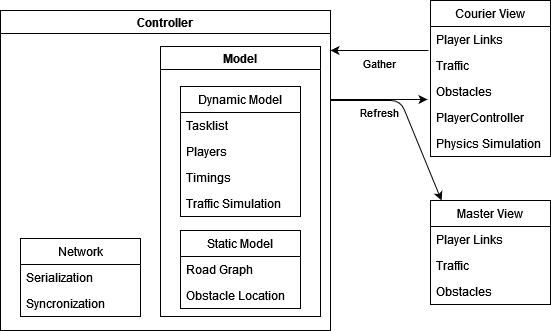
\includegraphics[width=\textwidth]{game architecture}
\subsection{Optimizations Techniques}
Culling, LODs, events

\clearpage

\section{Design}

\subsection{Game Design}
The game is set in a city, with gridstyle roads.
There are up to 2 couriers, which have to fulfil a list of delivery orders.
There is a master player who has a map, which shows the courier's positions and the streets status. The master has the order list, the couriers do not.
The orders consist of a pickup site and dropoff site.
The streets are blocked by many obstacles:
\begin{itemize}
  \item variable level of traffic makes the street difficult to navigate
  \item a drawbridge over a river or a rail
  \item a rail passage getting closed when a train crosses
\end{itemize}
The master has to plan the route during the time and relay the path to each courier in the broadcast channel.
The master's map is outfitted with a shortest path algorithm to ease finding a fast route.
The couriers drive following the Master path, they only see the pickup points and if they have picked up an item, the corrisponding dropoff point.

\subsection{Traffic simulation}
The traffic simulation can be tuned to different levels of complexity.
\subsubsection{Static}
The streets are filled with a random amount of immoble cars.
\subsubsection{Dynamic}
Every street has a traffic level associated to it. The traffic levels oscillate smoothly, but randomly over time. The cars are immoble, but when they are not seen by any players, the amount of cars in a street is adjusted to be proportional to the traffic level of the street.
\subsubsection{Agent Based}
The cars are agents that move thorugh a graph representation of the streets. The cars roam through the city by turning randomly at intersections. The cars respect traffic lights and obstacles on the streets, so that traffic jams happen dynamically.

\subsection{Variations}
\subsubsection{Events}
Throughout the city there are billboards and signs that contain the time and place an event will happen. The event (for example a parade, a festival, the street market, a strike) generates a lot of foot traffic and car traffic in a particular place. The master has no information about these events, so he has to rely on the couriers who will see the billboards and relay the information.
\subsubsection{Delivery Timers}
The delivery orders may have up to three additional timers: a time after which the order is failed if it's not picked up, a delivery time constraint and a time after which the order is failed if not completed.

\subsection{Master's Information}
The information that the master has of the players can be reduced in the settings. The master has three channels of information: geolocalization, video feed and audio from the radio. Turning off any of these channels the game becomes significantly harder, except when turning off the radio. The radio is essential for completing the game, so it cannot be switched off. A chatting system may substitute it partially.

\subsection{Interface Design}

\subsection{Syncronization model}
The game's state is split in static state and dynamic state. The static state is comprised of the data that does not change during the game and thus is syncronized only at the start of the game. The dynamic state instead is all the data that needs to be syncronized every tick. 
Every tick, which are a few milliseconds apart, each client sends their position to the server. The server integrates the positions in it's state and computes the next state, which is sent back to the clients.
 This approach has the advatage that it's naturally resilient to packet loss as the whole state is sent each time. Moreover, there is no network lag on the client character.
 The approach however has the disadvantage that it's weak against cheating, as the server trusts the position given by the client. This can be solved by running the simulation on the server to check for anomalies or by running it exclusively on the server, gathering the raw inputs of the clients instead of the position.

\smallskip
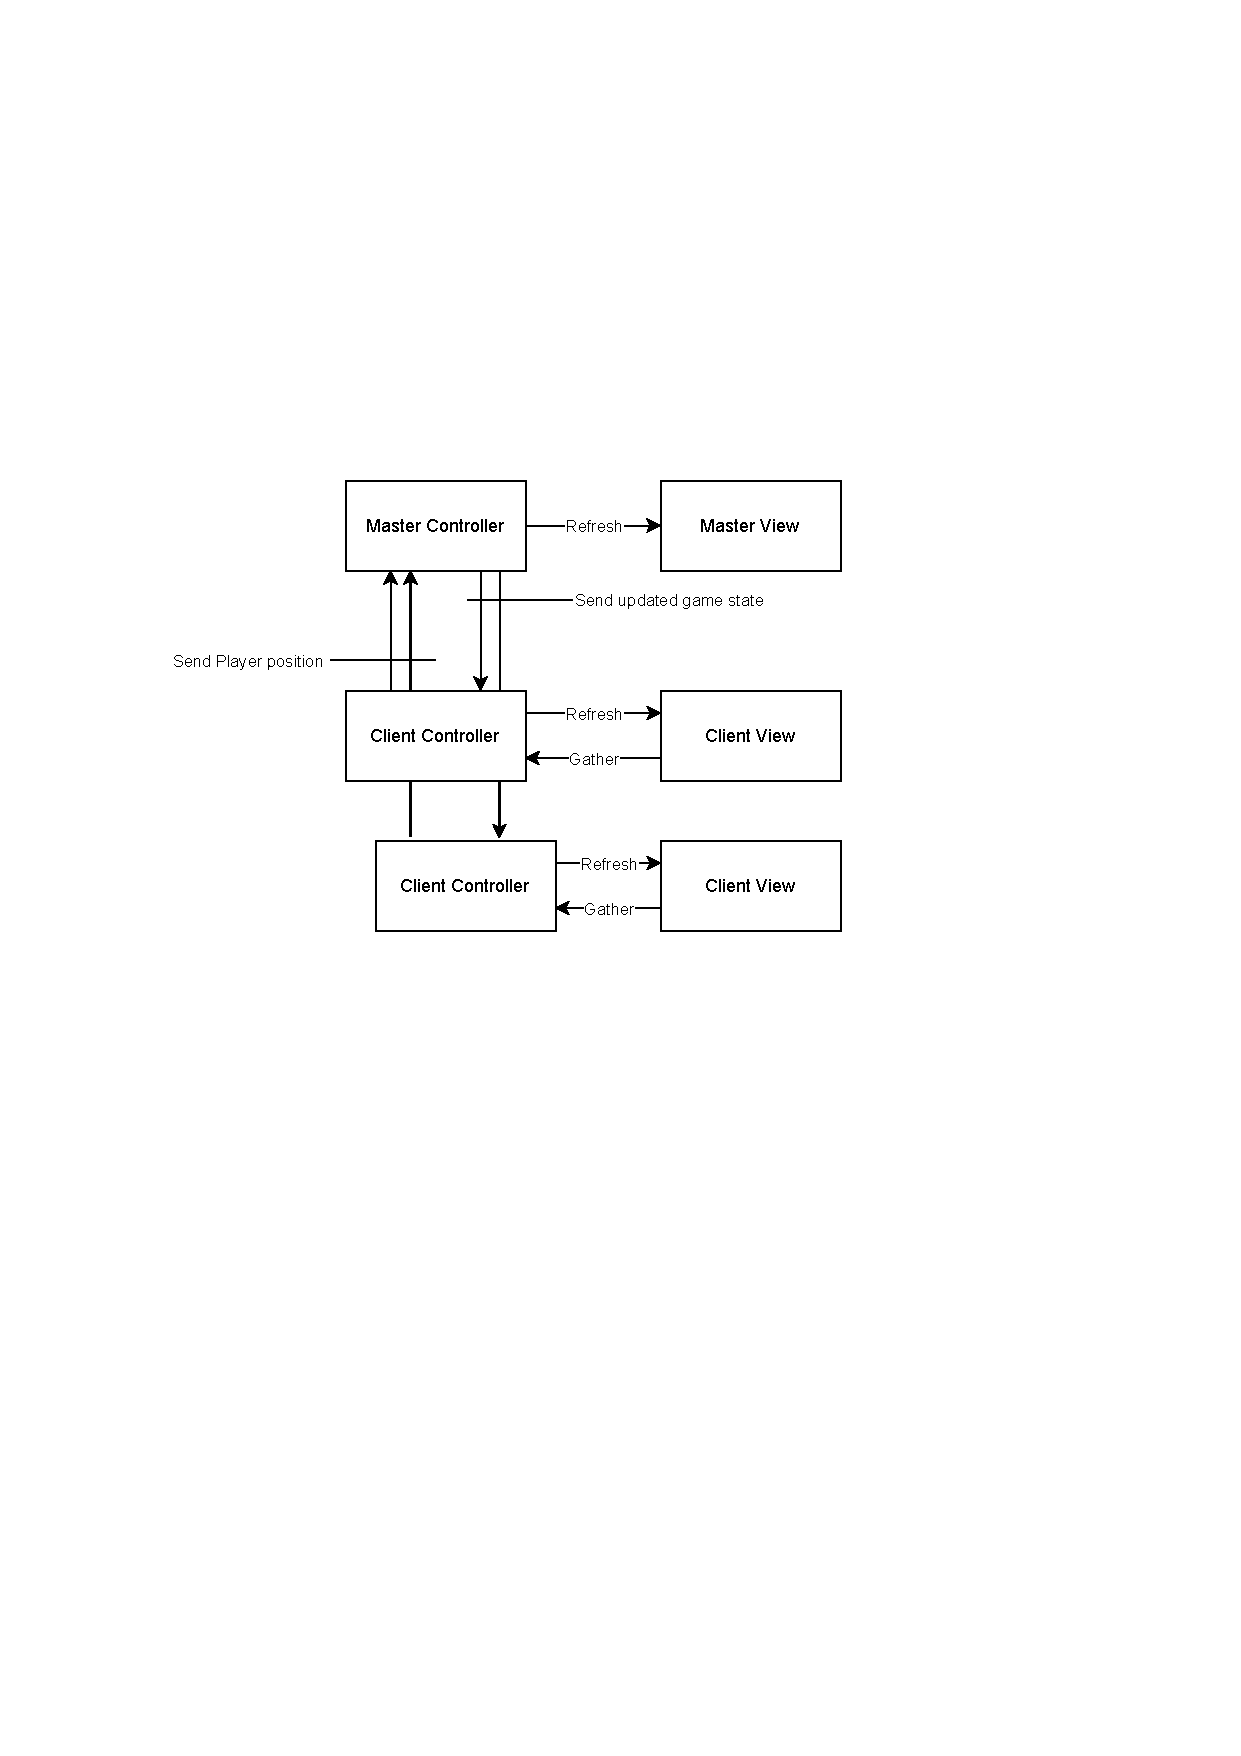
\includegraphics[width=\textwidth]{net architecture}

\smallskip
The static state is constructed by using the configuration of the lobby. In the lobby of the game, the master has the possibility to change map, set the number of tasks, set the available time and  turn off video feed and geolocalization. The changes are seen by all clients.

\subsection{Radio}
The radio in the game is a simulation of a real half-duplex radio. This means that only one player at the time may speak. This is enforced by transmitting white noise while two ore more player are using the radio channel.
\subsection{Video}
The video feed is a frame of the player's camera which is sent to the master by each player. The amount of data required scales rapidly with the resolution of the frame and the frequency of the transmission.

\clearpage

\section{Testing}
\subsection{Unit Testing and TDD}
The model of the game is developed using the test driven development technique. This technique allows writing testable code by first writing a failing test and then the code to pass it. This makes the code more robust and easier to clean. Other aspect of the game such as the controller, the view or the map tools are not easily testable this way as they depend on the unity framework. 
\subsection{Integration Testing}
The integration testing phase is largely done by hand. This is necessary as unity does't have a way to run multiple deployed instances inside a test environment, the testing routine is to deploy an executable and run it parallel to the editor instance. Some components are tested automatically, such as the serialization of the model and the interaction between smaller model components.

\clearpage
\bibliographystyle{plain}
\bibliography{references}

\end{document}